\documentclass[11pt]{article}
% Exercises figures, tables and equations with the packages people use most.
\usepackage[margin=1in]{geometry}
\usepackage{graphicx}
\usepackage{amsmath}
\usepackage{amssymb}
\usepackage{booktabs}
\usepackage{multirow}
\usepackage{longtable}
\usepackage{xcolor}
\usepackage{float}
\usepackage{caption}
\usepackage{subcaption}
\usepackage{cite}
\usepackage{hyperref}

\title{Rendering Check: Figures, Tables and Equations}
\author{PaperDesk Test Suite}
\date{}

\begin{document}
\maketitle

\section{Figures}
Figure~\ref{fig:plot} is a PNG, Figure~\ref{fig:photo} a JPEG and Figure~\ref{fig:diagram} a vector PDF.
Figure~\ref{fig:pair} shows two subfigures, one loaded from a nested folder~\cite{knuth1984,lamport1994}.

\begin{figure}[H]
  \centering
  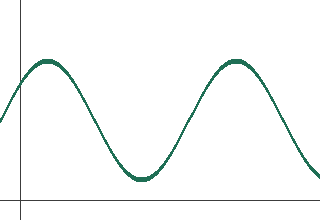
\includegraphics[width=0.6\linewidth]{figures/plot.png}
  \caption{A PNG line plot scaled to sixty percent of the line width.}
  \label{fig:plot}
\end{figure}

\begin{figure}[htbp]
  \centering
  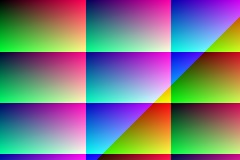
\includegraphics[scale=0.8]{figures/photo.jpg}
  \caption{A JPEG photograph at scale 0.8.}
  \label{fig:photo}
\end{figure}

\begin{figure}[htbp]
  \centering
  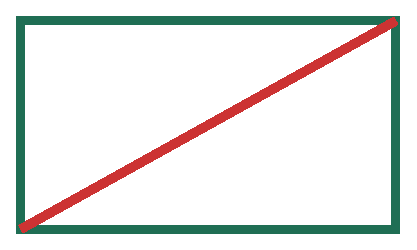
\includegraphics[width=\linewidth]{figures/diagram}
  \caption{A vector PDF diagram at full line width, referenced without its extension.}
  \label{fig:diagram}
\end{figure}

\begin{figure}[htbp]
  \centering
  \begin{subfigure}{0.45\linewidth}
    
\includegraphics[width=\linewidth]{figures/sub/gradient.png}
    \caption{Nested folder}
    \label{fig:pair-a}
  \end{subfigure}\hfill
  \begin{subfigure}{0.45\linewidth}
    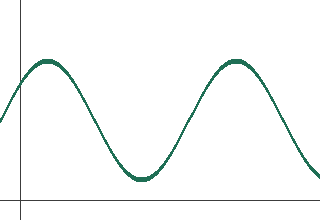
\includegraphics[width=\linewidth]{figures/plot.png}
    \caption{Same plot}
    \label{fig:pair-b}
  \end{subfigure}
  \caption{Two subfigures: \subref{fig:pair-a} and \subref{fig:pair-b}.}
  \label{fig:pair}
\end{figure}

\section{Tables}
Table~\ref{tab:basic} is a plain tabular, Table~\ref{tab:booktabs} uses \texttt{booktabs},
Table~\ref{tab:merged} merges cells and Table~\ref{tab:wide} is wider than the text block.

\begin{table}[H]
  \centering
  \caption{A basic tabular with rules.}
  \label{tab:basic}
  \begin{tabular}{|l|c|r|}
    \hline
    Item & Count & Price \\ \hline
    Apples & 3 & 1.20 \\
    Pears & 12 & 0.85 \\ \hline
  \end{tabular}
\end{table}

\begin{table}[htbp]
  \centering
  \caption{Booktabs rules.}
  \label{tab:booktabs}
  \begin{tabular}{lrr}
    \toprule
    Method & Accuracy (\%) & Time (s) \\
    \midrule
    Baseline & 81.2 & 4.1 \\
    Ours & \textbf{\color{teal}88.6} & 3.7 \\
    \bottomrule
  \end{tabular}
\end{table}

\begin{table}[htbp]
  \centering
  \caption{Multirow and multicolumn cells.}
  \label{tab:merged}
  \begin{tabular}{llcc}
    \toprule
    & & \multicolumn{2}{c}{Score} \\
    \cmidrule(lr){3-4}
    Group & Model & Dev & Test \\
    \midrule
    \multirow{2}{*}{Small} & A & 70.1 & 69.4 \\
                           & B & 72.3 & 71.0 \\
    \multirow{2}{*}{Large} & C & 80.5 & 79.9 \\
                           & D & 83.2 & 82.7 \\
    \bottomrule
  \end{tabular}
\end{table}

\begin{table}[htbp]
  \centering
  \caption{A wide table shrunk to the line width.}
  \label{tab:wide}
  \resizebox{\linewidth}{!}{%
  \begin{tabular}{lcccccccccc}
    \toprule
    Dataset & Jan & Feb & Mar & Apr & May & Jun & Jul & Aug & Sep & Total \\
    \midrule
    North region measurements & 101 & 98 & 110 & 120 & 131 & 140 & 151 & 149 & 133 & 1133 \\
    South region measurements & 88 & 91 & 95 & 102 & 118 & 125 & 129 & 127 & 119 & 994 \\
    \bottomrule
  \end{tabular}}
\end{table}

\begin{longtable}{rlr}
  \caption{A long table that spans pages.}\label{tab:long} \\
  \toprule
  Row & Label & Value \\
  \midrule
  \endfirsthead
  \toprule
  Row & Label & Value \\
  \midrule
  \endhead
  \bottomrule
  \endfoot
  1 & alpha & 0.10 \\ 2 & beta & 0.20 \\ 3 & gamma & 0.30 \\ 4 & delta & 0.40 \\ 5 & epsilon & 0.50 \\
  6 & zeta & 0.60 \\ 7 & eta & 0.70 \\ 8 & theta & 0.80 \\ 9 & iota & 0.90 \\ 10 & kappa & 1.00 \\
  11 & lambda & 1.10 \\ 12 & mu & 1.20 \\ 13 & nu & 1.30 \\ 14 & xi & 1.40 \\ 15 & omicron & 1.50 \\
  16 & pi & 1.60 \\ 17 & rho & 1.70 \\ 18 & sigma & 1.80 \\ 19 & tau & 1.90 \\ 20 & upsilon & 2.00 \\
  21 & phi & 2.10 \\ 22 & chi & 2.20 \\ 23 & psi & 2.30 \\ 24 & omega & 2.40 \\ 25 & aleph & 2.50 \\
  26 & beth & 2.60 \\ 27 & gimel & 2.70 \\ 28 & daleth & 2.80 \\ 29 & hbar & 2.90 \\ 30 & ell & 3.00 \\
  31 & wp & 3.10 \\ 32 & Re & 3.20 \\ 33 & Im & 3.30 \\ 34 & partial & 3.40 \\ 35 & infty & 3.50 \\
  36 & nabla & 3.60 \\ 37 & forall & 3.70 \\ 38 & exists & 3.80 \\ 39 & emptyset & 3.90 \\ 40 & angle & 4.00 \\
  41 & top & 4.10 \\ 42 & bot & 4.20 \\ 43 & flat & 4.30 \\ 44 & natural & 4.40 \\ 45 & sharp & 4.50 \\
  46 & clubsuit & 4.60 \\ 47 & diamondsuit & 4.70 \\ 48 & heartsuit & 4.80 \\ 49 & spadesuit & 4.90 \\ 50 & surd & 5.00 \\
  51 & prime & 5.10 \\ 52 & triangle & 5.20 \\ 53 & neg & 5.30 \\ 54 & backslash & 5.40 \\ 55 & Box & 5.50 \\
\end{longtable}

\section{Equations}
Inline math such as $e^{i\pi} + 1 = 0$ and $\alpha \leq \beta \in \mathbb{R}$ sits in the text.
A display without a number:
\[
  \int_0^\infty e^{-x^2}\,dx = \frac{\sqrt{\pi}}{2}.
\]
A numbered equation:
\begin{equation}
  \label{eq:euler}
  \sum_{n=1}^{\infty} \frac{1}{n^2} = \frac{\pi^2}{6}
\end{equation}
An aligned system, numbered line by line:
\begin{align}
  f(x) &= (x+1)^2 \label{eq:square} \\
       &= x^2 + 2x + 1 \nonumber \\
  g(x) &\approx \mathcal{O}(x^3) \label{eq:cubic}
\end{align}
and an unnumbered one:
\begin{align*}
  \nabla \cdot \mathbf{E} &= \frac{\rho}{\varepsilon_0} &
  \nabla \times \mathbf{B} &= \mu_0 \mathbf{J}
\end{align*}
Matrices and cases:
\[
  A = \begin{pmatrix} 1 & 2 \\ 3 & 4 \end{pmatrix}, \quad
  B = \begin{bmatrix} a & b \\ c & d \end{bmatrix}, \quad
  |x| = \begin{cases} x & x \geq 0, \\ -x & x < 0. \end{cases}
\]
Equation~\eqref{eq:euler} is the Basel problem, \eqref{eq:square} expands a square and
equation~\ref{eq:cubic} is cubic. Symbols: $\forall\, \exists\, \emptyset\, \subseteq\, \mathbb{N}\, \mathbb{Z}\, \therefore\, \leqslant\, \geqslant\, \nexists$.

\begin{thebibliography}{9}
\bibitem{knuth1984} D.~E. Knuth, \emph{The \TeX book}, Addison-Wesley, 1984.
\bibitem{lamport1994} L.~Lamport, \emph{\LaTeX: A Document Preparation System}, 2nd ed., 1994.
\end{thebibliography}

\end{document}
